\section{商业模式设计流程}

商业模式设计流程有五个阶段:\textbf{动员}、\textbf{理解}、\textbf{设计}、\textbf{实施}和\textbf{管理}。

\subsection{商业模式创新的基本出发点}

商业模式创新的目的无非以下四种:
\begin{itemize}
    \item 满足市场:满足未被响应的市场需求。比如印度塔塔汽车、私人飞机租赁商奈特捷、孟加拉乡村银行、鲁鲁自助出版社(lulu.com)。
    \item 投放市场:将新技术、产品或服务推向市场,或者开发现有的知识资产。比如施乐914型 复印机、Swatch手表、Nespresso胶囊咖啡、红帽子开源软件公司。
    \item 改进市场:改进或者颠覆当前的市场。比如戴尔电脑公司、瑞士盈丰私人银行、任天堂Wii、宜家、印度巴蒂电信、Skype、瑞安航空、亚马逊零售业务、从事电动汽车电池服务的乐土公司。
    \item 创造市场:创造一种全新的业务。比如大来卡就餐信用卡、谷歌。
\end{itemize}

上述过程所面对的挑战有:
\begin{itemize}
    \item 找到正确的模式
    \item 在全面启动前验证该模式
    \item 诱导市场接受新的模式
    \item 根据市场的反馈不断调整该模式
    \item 管理不确定因素
\end{itemize}

对于成熟企业来说,商业模式创新活动通常反映了它当前的商业模式和组织结构。它们的创新通常会缘 于以下四种动机之一:
\begin{itemize}
    \item 被动反应:由当前商业模式的危机而引发。比如20世纪90年代的IBM、任天堂的Wii、劳斯莱斯喷气引擎。
    \item 调整适应:调整、改进或者捍卫现有的商业模式。比如诺基亚的“与音乐同行Comeswithmusic”项目、宝洁公司的开放创新计划、建筑行业产品制造商喜利得公司。
    \item 扩张:发布一项新技术、产品或者服务。比如Nespresso胶囊咖啡、20世纪60年代的施乐914复印机 、iPod/iTunes
    \item 主动开拓:为未来做准备。比如戴姆勒的Car2go、亚马逊云计算服务AmazonWebService。
\end{itemize}


上述过程所面对的挑战有:
\begin{itemize}
    \item 对新的模式产生欲望
    \item 新老模式之间的拉通
    \item 管理既得利益
    \item 聚焦长远利益
\end{itemize}

\subsection{设计态度}
\begin{itemize}
    \item 创新的参与者必须愿意投入大量的时间和经历去探索很多的可能,而不是过早地采用某一种解决方案,时间的投入会得到回报的,会因此获得更强大的新商业模式,确保未来的增长。
    \item 寻找真正出色的方案,而不是修饰一个很快得到的方案。
\end{itemize}

\begin{figure}[H]
	\centering
	\vspace{-0.5em}
	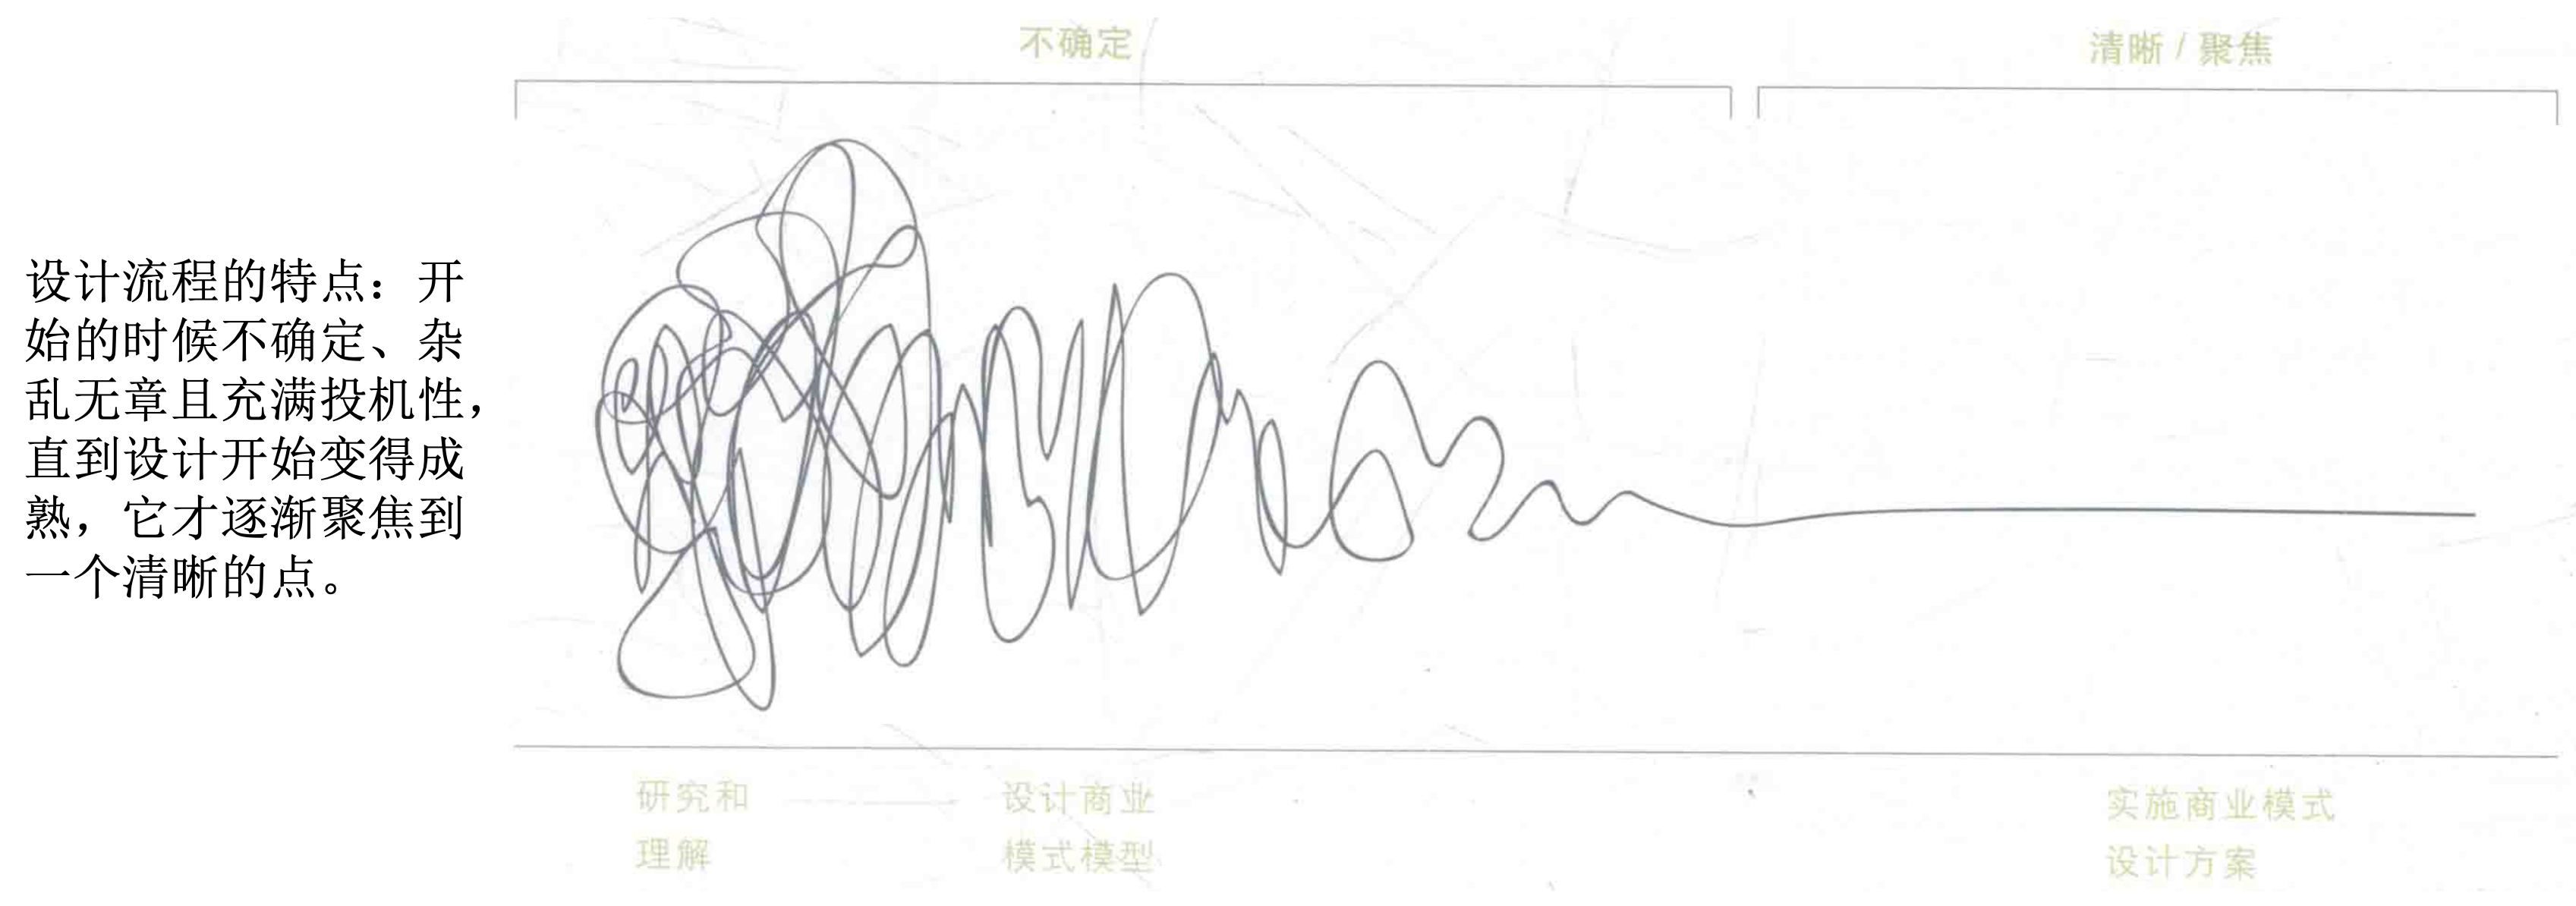
\includegraphics[width=0.7\textwidth]{img/设计曲线.png}
    \vspace{-0.5em}
\end{figure}

\subsection{商业设计流程的五个阶段}

\begin{figure}[H]
	\centering
	\vspace{-0.5em}
	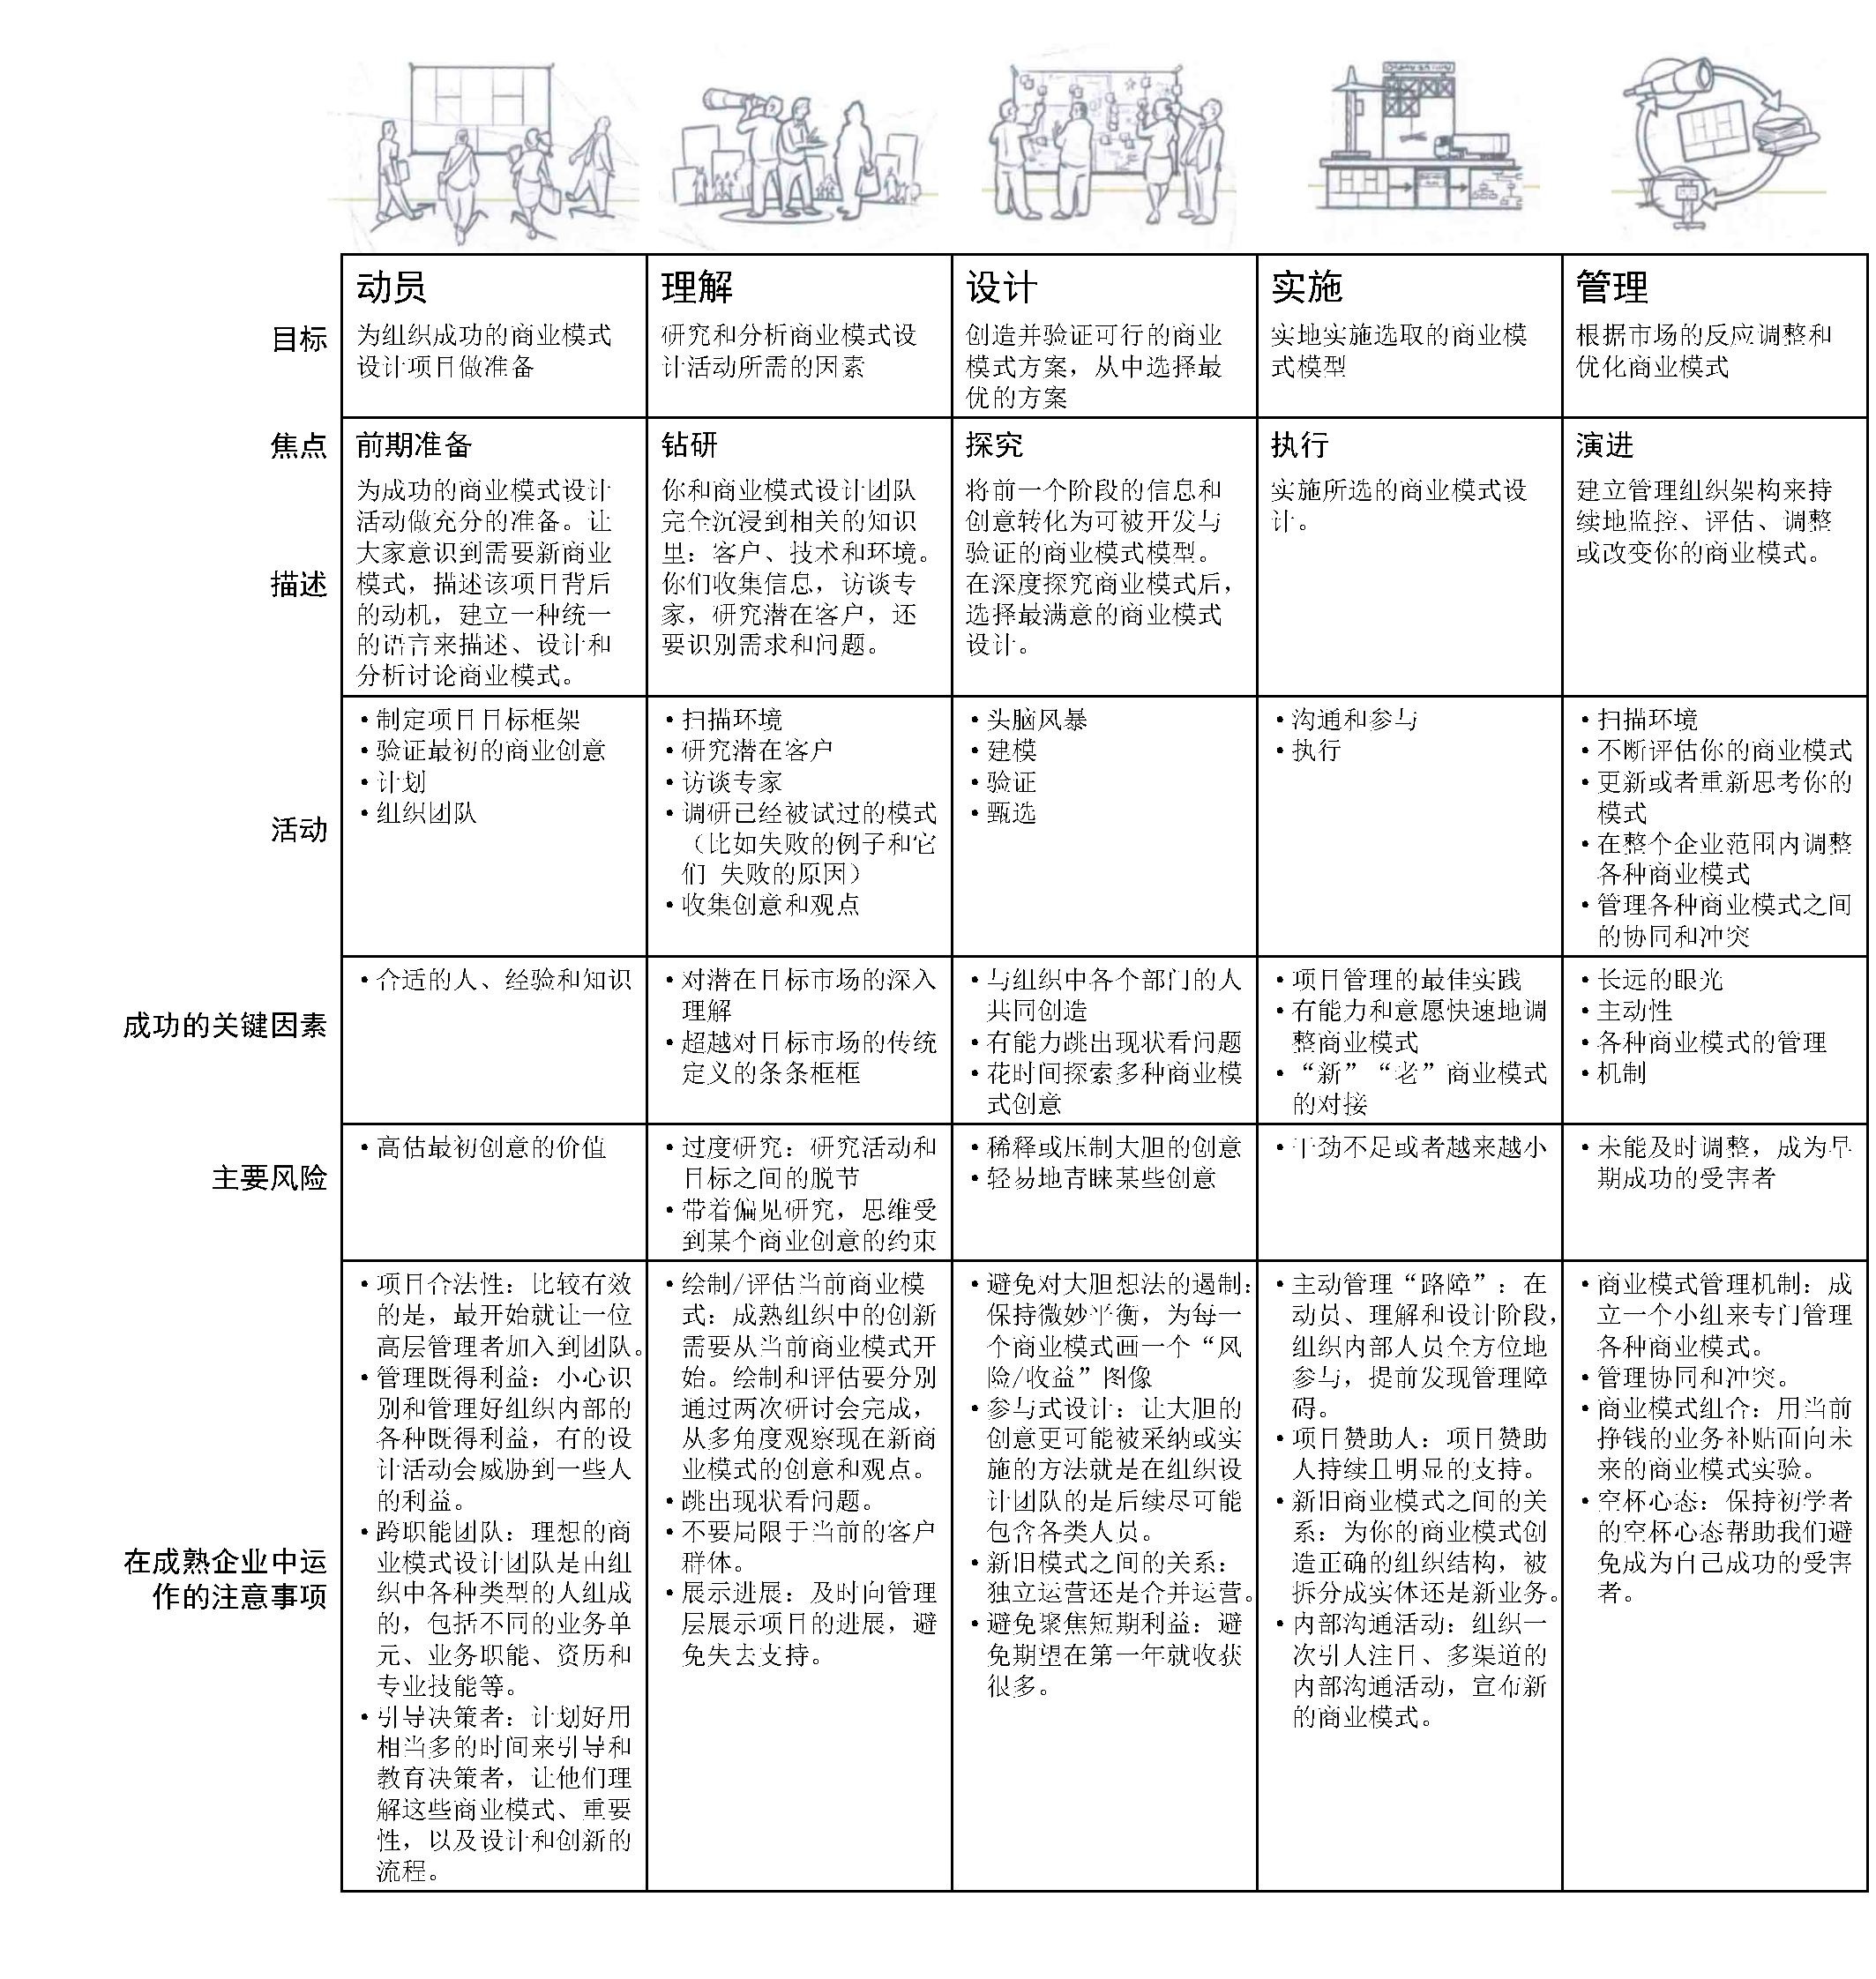
\includegraphics[width=\textwidth]{img/商业模式设计流程.pdf}
    \vspace{-0.5em}
\end{figure}

